\documentclass[conference]{IEEEtran}

\usepackage[pdftex]{graphicx}
\usepackage[utf8]{inputenc} % Diacritics and special letters.
\usepackage[T1]{fontenc} % Encoding table for characters.
\usepackage{flushend}

\begin{document}

%-------------------------------------------------------------------------
\title{Heterogeneous Hybrid Networks Reliability Simulation}
%-------------------------------------------------------------------------

%TODO other possible tiles
% Simulation Platform and Scenario Generator for Time-Triggered Wired/Wireless Networks
% Simulation Platform and Scenario Generator for Wired/Wireless Networks with Mixed Time and Reliability Requirements

%TODO other possible title wordings
% -Simulation
% -Platform, toolchain, environment
% -Time-triggered, TDMA, mixed-traffic requirements
% -Ethernet-based
% -Hybrid, wired/wireless networks
% -Scenarios generation

\author{
\IEEEauthorblockN{Pablo Gutiérrez Peón\IEEEauthorrefmark{1}\IEEEauthorrefmark{2},
Francisco Pozo\IEEEauthorrefmark{2}, Guillermo Rodriguez-Navas\IEEEauthorrefmark{2}}

\IEEEauthorblockA{\IEEEauthorrefmark{1}TTTech Computertechnik AG, Vienna, Austria}

\IEEEauthorblockA{\IEEEauthorrefmark{2}School of Innovation, Design and Engineering, Mälardalen University, Västerås, Sweden\\
Email: pablo.gutierrez-peon@tttech.com, francisco.pozo@mdh.se, guillermo.rodriguez-navas@mdh.se}}

\maketitle

%-------------------------------------------------------------------------
%\begin{abstract}
%-------------------------------------------------------------------------

%The use of computer simulations can help to evaluate the performance of real-time data networks and detect potential issues that compromise the ultimate goal of providing timely and reliable communications. A theoretical analysis over components of the communication system such as the physical layer, medium access, or routing, is too complex or only able to cover pessimistic cases. Further, simulations must include all aspects that are relevant for the performance evaluation. Wireless communication is subject to phenomena like fading, shadowing, etc. which are not always included in simulations. Still, advantages like mobility, flexibility in the deployment or reduced cost and weight might trigger the consideration of wireless communications. Instead of completely replacing wired links, wireless links are often seen as a complement to wired networks, enabling new application domains. At the same time, there is a trend towards the convergence between networks for industrial, automotive or aerospace fields serving real-time requirements and networks for office and home environments that focus on throughput at the cost of offering a best-effort service. Important to mention is that message scheduling is crucial in the design of a real-time communication systems. Unlike event-triggered message dispatching, in the time-triggered paradigm the instants when transmissions are done are pre-defined, having the advantage that the behaviour of scheduled message transmissions are always known which simplifies its safety certification. Unfortunately, accessing the medium does not guarantee that the message will be delivered. Although absolute guarantees cannot be given, simulation can help to evaluate if sufficient reliability is provided for the transmissions and if the timing requirements can be kept.

%The use of computer simulations can help to evaluate the performance of real-time data networks and detect potential issues that compromise the ultimate goal of providing timely and reliable communications. A theoretical analysis over components of the communication system such as the physical layer, medium access, or routing protocols might be too complex or only able to cover pessimistic cases. Further, simulations must include all aspects that are relevant for the performance evaluation. In our case, we are interested in simulating hybrid wired/wireless networks, with special focus on emulating problems like fading, shadowing or interference, which are typically disregarded in wired links. Despite these problems, advantages like mobility, flexibility in the deployment or reduced cost and weight might trigger the consideration of wireless communications. Instead of completely replacing wired links, wireless links are often seen as a complement to wired networks, enabling new application domains. A crucial aspect in the design of a real-time communication system is message scheduling. Even so, a schedule that guarantees the access to the medium does not assure that the message will be delivered. Although absolute guarantees cannot be given, simulation can help to evaluate if sufficient reliability is provided for the transmissions and if the timing requirements can be kept. 

%This work aims at providing a simulation platform to test hybrid wired/wireless networks where both time-triggered real-time and non-real-time traffic travel seemingly over different transmission media.

This work aims at providing a novel tool HeNReS (Heterogeneous Hybrid Networks Reliability Simulation) to test the reliability of hybrid wired/wireless networks were both time-triggered real-time and non-real-time traffic travel seemingly over different transmission media. Nowadays, the inherent diversity of these networks makes the analysis more complex, specially with the addition of wireless links, susceptible to problems like fading, shadowing or interference, which are typically disregarded in wired links. A simulation of these networks usually requires the cooperation of multiple tools that do not share the same input/output interfaces. Our simulation tool facilitates this process providing integrated state-of-the-art tools where the user only needs to provide a set of simulation parameters in a single file to obtain the reliability of the network. The simulation tool is executed using a \textit{makefile} that will perform a different simulation for every set of parameters given and returns performance measures in terms of reliability and message delays among others.

%This work aims at providing a simulation platform to test hybrid wired/wireless networks where both time-triggered real-time and non-real-time traffic travel seemingly over different transmission media. The simulation platform proposed in this work consists of four main software components: network and traffic generator, traffic scheduler, network simulator and results processing. Each software component uses a file or set of files to interface with other components.



Internally, the simulation platform consists of four main software components: network and traffic generator, traffic scheduler, network simulator and results processing. In Figure \ref{fig:toolchain-architecture} we can see how each software component interfaces with others using a file or set of files. In the next paragraphs we go more into detail into the function of each component.

The network and traffic generator is able to create any non-cyclic network topology with different traffic profiles. Note that it is possible to specify more than one network and traffic, which will create multiple simulation configurations. The network is composed of four types of devices: wired end-systems, wireless end-systems, switches and access points. End-systems are responsible to send and receive traffic, while switches and access points relay messages through the network, creating multi-hop paths between end-systems. Access points serve to interface between wired and wireless media. The traffic is generated in form of messages, containing information of its size, period and deadline, that can be sent from one end-system to any group of end-systems of the network.

%The network and traffic generator is capable of producing the network topology and incorporate different traffic profiles defined by the user in a configuration file. The network is composed of four types of devices: wired end-systems, wireless end-systems, switches and access points. Wired end-systems and wireless end-systems are responsible to send and receive traffic and only differ between each other with the capabilities of receiving wireless communication for the wireless end-systems. Switches are responsible of relaying the messages through the network, creating multi-hop paths between end-systems, while access points, connected to a switch, transmit and receives messages in the wireless medium to and from wireless end-systems. The traffic is generated in form of messages, containing information of its size, period and deadline, that can be sent from one end system to any group of end systems of the network.

The traffic scheduler implements a scheduling algorithm capable of generating schedules for large and complex networks. It is developed using a combination of segmentation approaches and a Satisfiability Modelo Theory (SMT) Solver. It takes as input the network and traffic generated before-hand and assigns the transmission times for all the real-time messages in the network while satisfying its constraints. In the case of non-real-time traffic, it is handled at runtime by the network simulator.

The network simulator is developed in the OMNeT++ discrete event simulation framework. The basic components of an OMNeT++ simulation are the modules, the pieces where the functionality is implemented. Modules are connected to each other using gates and exchange information using message passing. The modules are partially described using the NED language from OMNeT++, that specifies the parameters, gates and nested modules, while the functionality is programmed in C++. The OMNeT++ initialization file is used to give value to the module parameters. The values can be grouped with labels that define different configurations, each specifying a set of values for the module parameters. The four types of network devices are able to dispatch messages in a time-triggered manner following the corresponding link schedule while non-real-time traffic can dynamically take the remaining time. The wired and wireless devices are based on IEEE 802.3 and IEEE 802.11 respectively, with a modified medium access control (MAC) layer. Inside the MAC, queues are FIFO, and traffic of different classes is segregated into different queues. Several mechanisms are incorporated to increase the reliability of wireless links, including retransmissions and cognitive radio. To test the reliability of the wireless links, interference emulating Carrier Sense Multiple Acess (CSMA) and jamming at different levels of intensity, size of burst and frequency hopping is contemplated. The simulation can run with a graphical environment or using the command line. The network simulator provides results in three types of files: scalar and vectorial result files and log file. Scalar and vectorial result files retrieve statistics and vectors of raw data, including, e.g., number of packets sent and received, the instants when those packets are sent, the MAC to MAC delay, defined as the time between a message, is made available in the MAC of the source node until it reacher the MAC of the destination node. It serves to evaluate the overhead introduced by the MAC. For reliability, the result is provided in the form of percentage of successful message transmissions.. The log file includes entries about communication events (e.g., message sent/received) and the time at which they happened.

The results processing tool takes the simulation log file as an input and creates a report after evaluating whether the logic and timing of the events is according to the MAC protocol design and the schedule.

%In order to facilitate the use of the simulation tool, a single file records all the parameters required by the user. To build the set of tools and run them, a makefile is created.

%TODO Motivation:
% - IT/OT, time-triggered, industrial networks

%TODO what do we offer:
% - Hybrid wired/wireless networks
% - Generates traffic and network topologies (describe how)
% - Built-in SMT traffic scheduler.
% - Network simulation. INI file can be modified to tune all the desired parameters.
% - Log checker tool.
% - TT traffic and BE
% - Wireless interferers
% - Reliability, delays (schedule is supposed to work, but here we check it)
% - Mechanisms for improved reliability (retransmissions, cognitive radio
% - Simulation made easy: one input file to generate several tests. Makefile: one instruction and wait for the results.

%TODO Describe the components of the simulator.

%TODO Describe what we have been able to achieve so far? I dont think we can use references.


%\end{abstract}

%TODO Make intro to the figures?

%TODO maybe add legend here

\begin{figure*}[h]
	\centerline{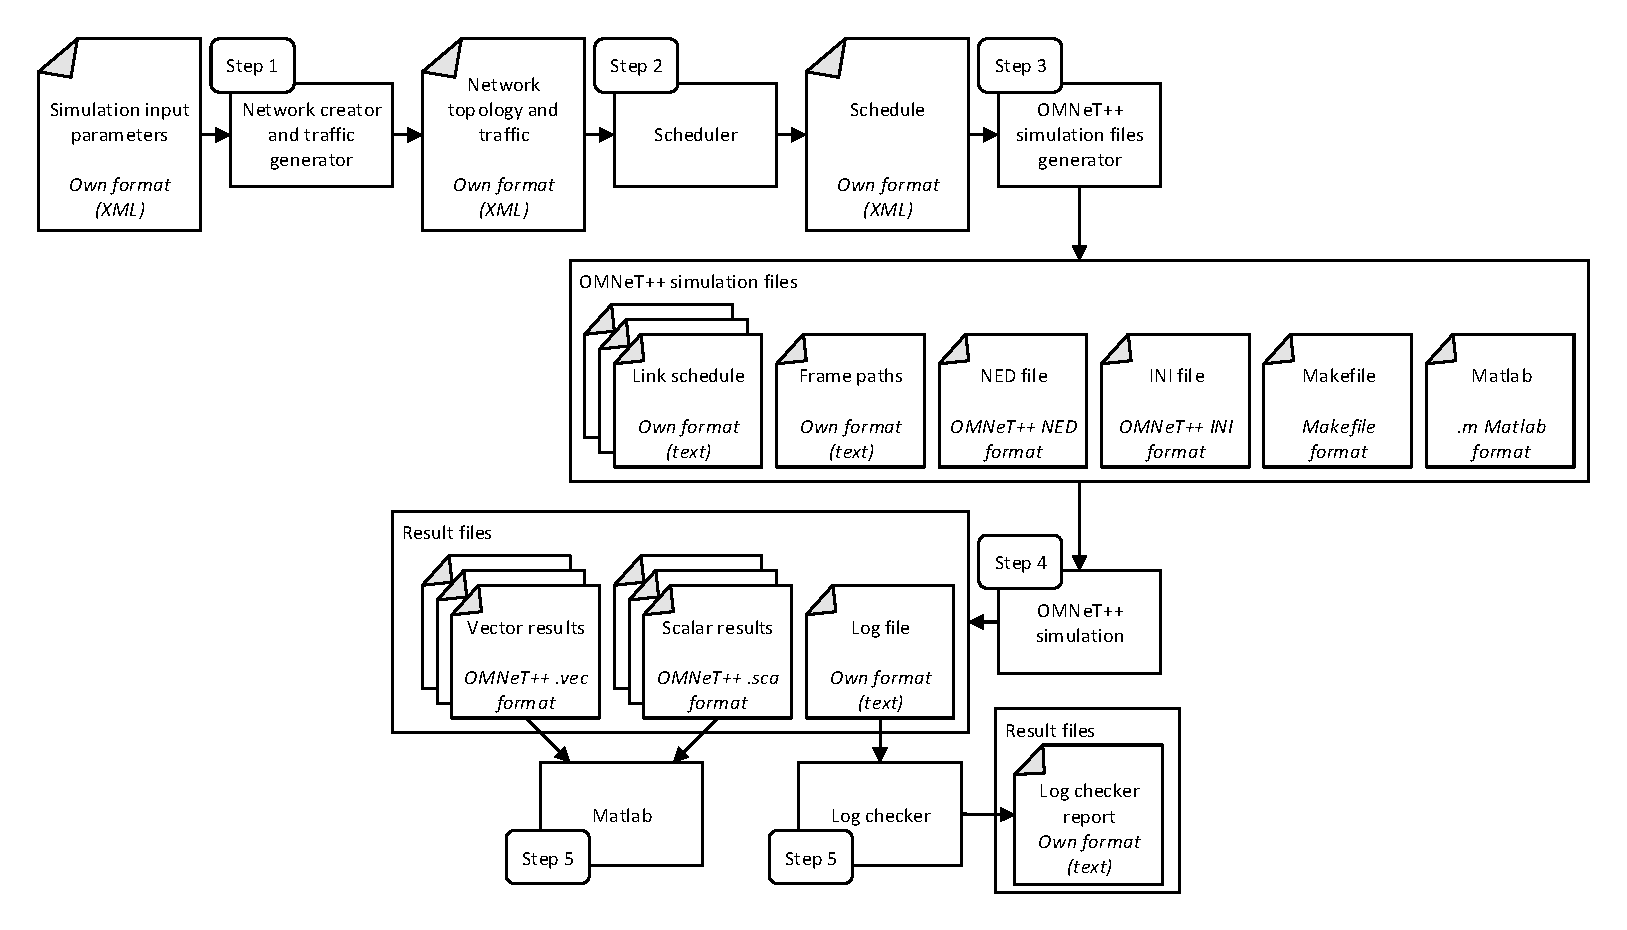
\includegraphics[keepaspectratio=true, width=16cm] {figures/toolchain-architecture}}
	\caption{Graphic representation of the tools flow implemented from the given simulation input up to getting the simulation results}
	\label{fig:toolchain-architecture}
\end{figure*}

\begin{figure*}[h]
	\centerline{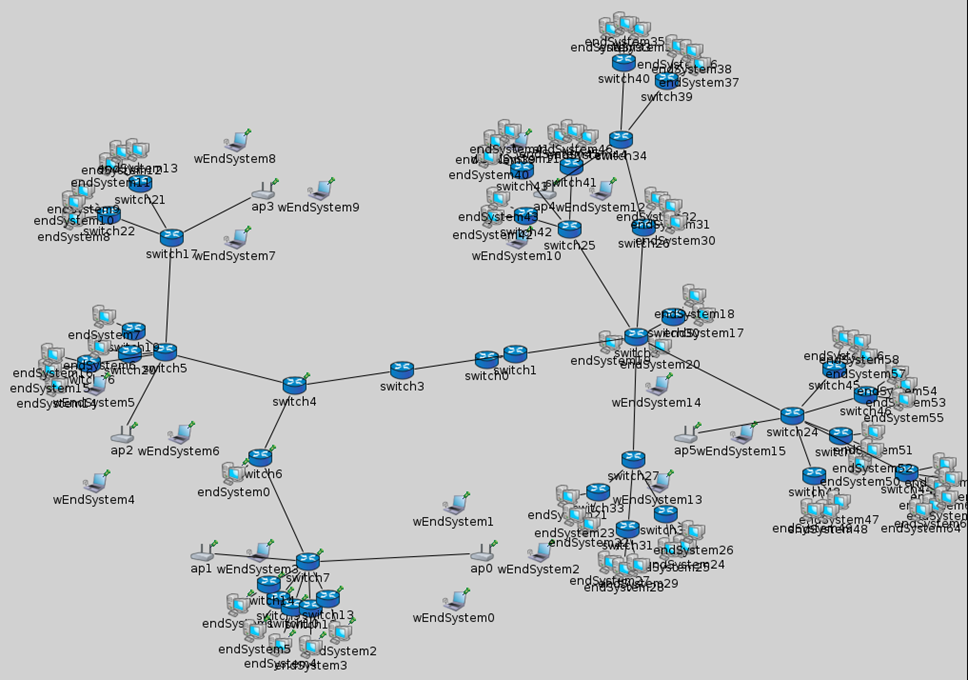
\includegraphics[keepaspectratio=true, width=16cm] {figures/s1-3}}
	\caption{Example of large network simulated containing 44 switches, 6 access points, 65 wired end systems, 16 wireless end systems, 212 wires dataflow links and 32 wireless dataflow links}
	\label{fig:s1-3}
\end{figure*}

\end{document}
